\documentclass{beamer}
\usepackage{listings}
\lstset{
%language=C,
frame=single, 
breaklines=true,
columns=fullflexible
}
\graphicspath{{./Figures/}}
\usepackage{gensymb}
\usepackage{subcaption}
\usepackage{url}
\usepackage{tikz}
\usepackage{tkz-euclide} % loads  TikZ and tkz-base
%\usetkzobj{all}
\usetikzlibrary{calc,math}
\usepackage{float}
\usepackage{extarrows}
\newcommand\norm[1]{\left\lVert#1\right\rVert}
\providecommand{\pr}[1]{\ensuremath{\Pr\left(#1\right)}}
\newcommand{\myvec}[1]{\ensuremath{\begin{pmatrix}#1\end{pmatrix}}}
\renewcommand{\vec}[1]{\mathbf{#1}}
\usepackage[export]{adjustbox}
\usepackage[utf8]{inputenc}
\usepackage{amsmath}
\usetheme{Boadilla}

\title{Construction of Quadrilateral with 2 sides and 3 angle}
\author{Sujal - AI20BTECH11020}

\date{\today}
\begin{document}

\begin{frame}
\titlepage
\end{frame}
\begin{frame}
\frametitle{Problem}
\begin{block}{Construct}
A quadrilateral $ABCD$ with given information
    \begin{align}
    &\angle A =  \alpha \label{eq 1}
    \\
    &\angle B =  \beta \label{eq 2}
    \\
    &\angle C = \gamma \label{eq 3}
    \\
    &\norm{\vec{A}-\vec{B}} = a \label{eq 4}
    \\
    &\norm{\vec{B}-\vec{C}} =  b \label{eq 5}
    \end{align}
\end{block}
\end{frame}

\begin{frame}
First, Consider
\begin{align}
\vec{A}=\myvec{0\\0},\vec{B}=\myvec{a\\0}
\end{align}
and calculate angle between $CD$ and +x-axis is $\theta$
\begin{align}
\theta &= 360\degree - (\beta + \gamma)\label{eq a}
\end{align}
and we have to find $\vec{C}$ and $\vec{D}$, which as shown in fig \ref{genralise}.
\begin{figure}[!h]
\centering
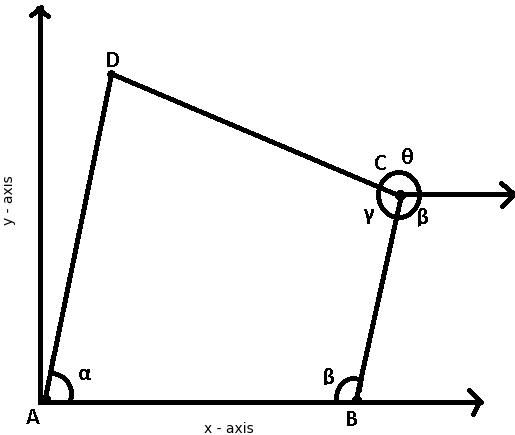
\includegraphics[ width=5cm]{plot_rough.png}
\caption{Quadrilateral MIST}
\label{genralise}	
\end{figure}
\end{frame}

\begin{frame}
\begin{lemma}
For $\vec{C}$, 
\begin{align}
\vec{C} =\vec{B} + b\vec{X} \text{ where } \vec{X} = \myvec{\cos (180\degree -\beta)\\\sin (180\degree -\beta)} \label{eq b}
\end{align}
here, $\vec{X}$ is unit vector in direction of line $BC$ and then multiply it with $b$ which is magnitude of line $BC$ and last adding $\vec{B}$. For $\vec{D}$,
\begin{align}
\vec{D} = x\vec{Y} \text{ where } \vec{Y} = \myvec{\cos\alpha\\\sin \alpha}\text{ and } x \in R^{+} \label{eq c}
\end{align}
Here, $\vec{Y}$ is unit vector in direction of line $AD$, and we need to find $x$ which is magnitude of line $AD$. Also, we use $\vec{C}$ to find $\vec{D}$ as 
\begin{align}
\vec{D} = y\vec{Z}+\vec{C} \text{ where } \vec{Z} =  \myvec{\cos\theta\\\sin\theta} \text{ and }y \in R^{+} \label{eq d}
\end{align}
Here, $\vec{Z}$ is unit vector in direction of line $CD$ and we need to find $y$ which is magnitude of line $CD$.
\end{lemma}
\end{frame}
\begin{frame}
Thus, 
from  \eqref{eq 2} and \eqref{eq 5} in \eqref{eq b}, we easily calculate $\vec{C}$ and from \eqref{eq c},\eqref{eq d} and $\vec{C}$, we get 
\begin{align}
&x\vec{Y} = y\vec{Z}+\vec{C}\\
&\myvec{\cos\alpha & -\cos\theta \\ \sin\alpha & -\sin\theta} \myvec{x \\ y} = \vec{C}
\end{align}
and then find $x$ and $y$\\
So, using $x$ and \eqref{eq c} we get $\vec{D}$
\end{frame}

\end{document}